\documentclass{article}
\usepackage[utf8]{inputenc}
\usepackage{fullpage}
\usepackage{graphicx}
\usepackage[T1]{fontenc}
\usepackage{amsmath}
\usepackage{float}
\title{Processing of images (2D signals)}
\author{Tajda Škraba (63180281)}
\date{}

\begin{document}

\maketitle {}

\textbf{Abstract} \newline
This seminar shows results of processing images using two different approaches. The original two-dimensional signals used in the seminar were first blurred and then sharpened. In the first approach we sharpened the images using the smoothing filter. The second approach for image sharpening used the second-order derivatives of an image which was obtained by using the Laplacian mask.
\section{Introduction}
Digital image processing is the conception, design, development, and enhancement of digital imaging programs \cite{io}.
Image sharpening is a useful tool when it comes to emphasising texture and drawing viewer attention. If done correctly, it can improve the image's quality. On the other hand, if done incorrectly or too aggressively, sharpening artifacts may appear. In the following section, we present the two methods used in this seminar.
\section{Methods}
We used MATLAB programming language for implementing our solution and the MathWorks Image Processing Toolbox \cite{ena} since it already contains all the functions we needed for this project. \newline
\newline
Before sharpening the images using the two different methods, we blurred the original images using a 3x3 kernel with values 1/9. We applied the filter to the original image using  $imfilter$ function \cite{dva}.
\subsection{Sharpening using smoothing filter}
In this method, we subtracted the blurred image from the original using the $imsubtract$ function \cite{tri} and added the result to the original image using the $imadd$ function \cite{stiri} multiple times. We repeated the addition $A$ times where $A > 1$. When $A\textgreater 1$ the filtering is called high boost filtering.
\subsection{Second-order derivatives for image sharpening}
This method used the Laplacian mask $\begin{bmatrix} 
1 & 1 & 1\\ 
1 & -8 & 1\\ 
1 & 1 & 1  
\end{bmatrix}$ to obtain the second derivative of an image, therefore the second-order derivatives were: \begin{equation}
g(x) = f(x,y) + \nabla^2f(x,y)
\end{equation} \newline where $f(x,y)$ is the original image, $g(x,y)$ is the sharpened image and $\nabla^2f(x,y)$ is an approximation of the second derivative of an image. Using the $conv2$ \cite{con} function, we performed the two dimensional convolution using the Laplacian mask and the original image and then we subtracted that from the blurred image to obtain the result.
\section{Results}
After the processing of the images with both methods, the results are shown in Figures 1 to 5. Because of different qualities of the original images, sharpening was more evident, for example Figures 1, 4 and 5.
\begin{figure}[H]
\centering
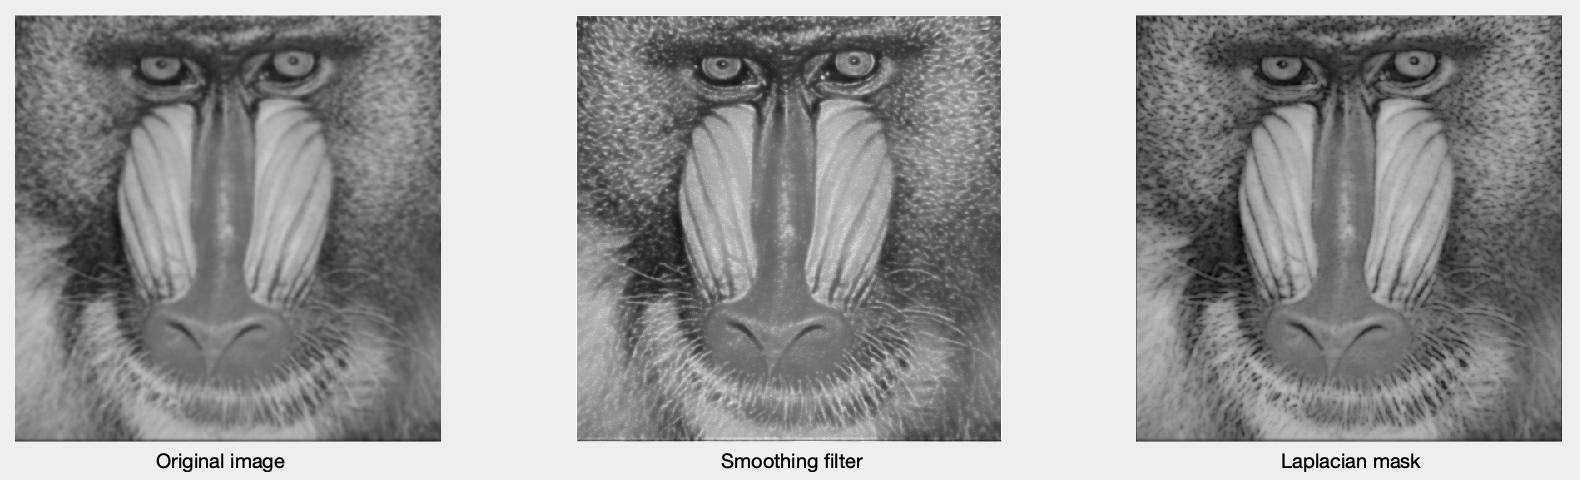
\includegraphics[width=\linewidth]{i.png}
\caption{Comparison of the original image with the sharpened images using both methods}
\label{fig:badLes}
\end{figure}
\begin{figure}[H]
\centering
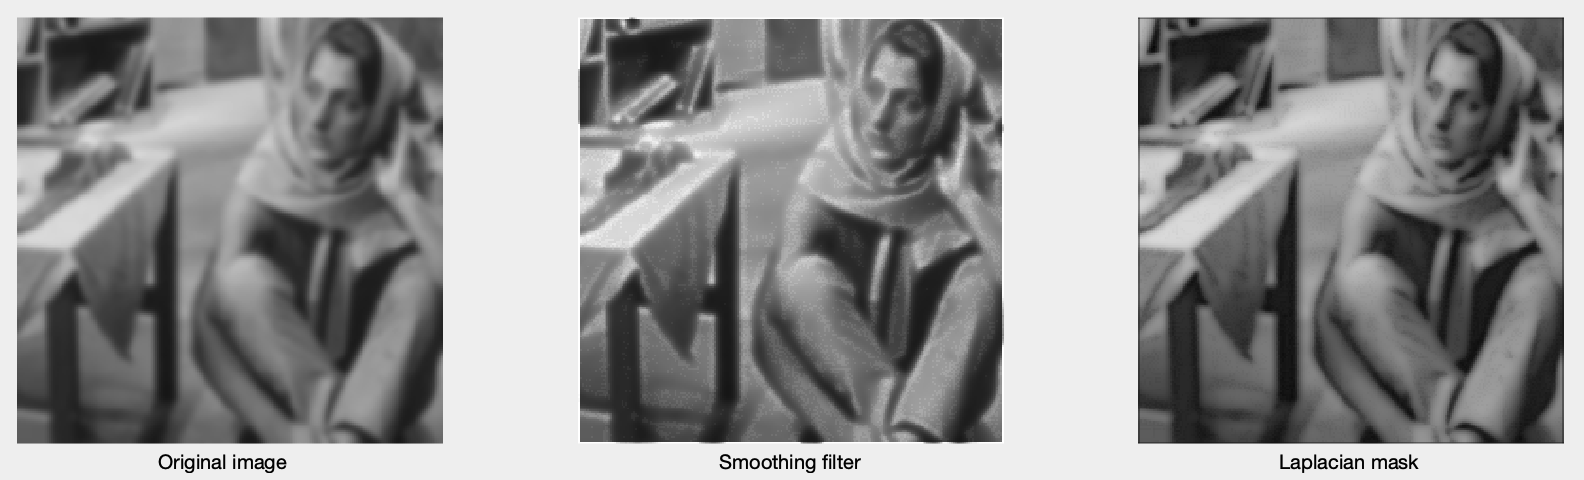
\includegraphics[width=\linewidth]{j.png}
\caption{Comparison of the original image with the sharpened images using both methods}
\label{fig:badLes}
\end{figure}

\begin{figure}[H]
\centering
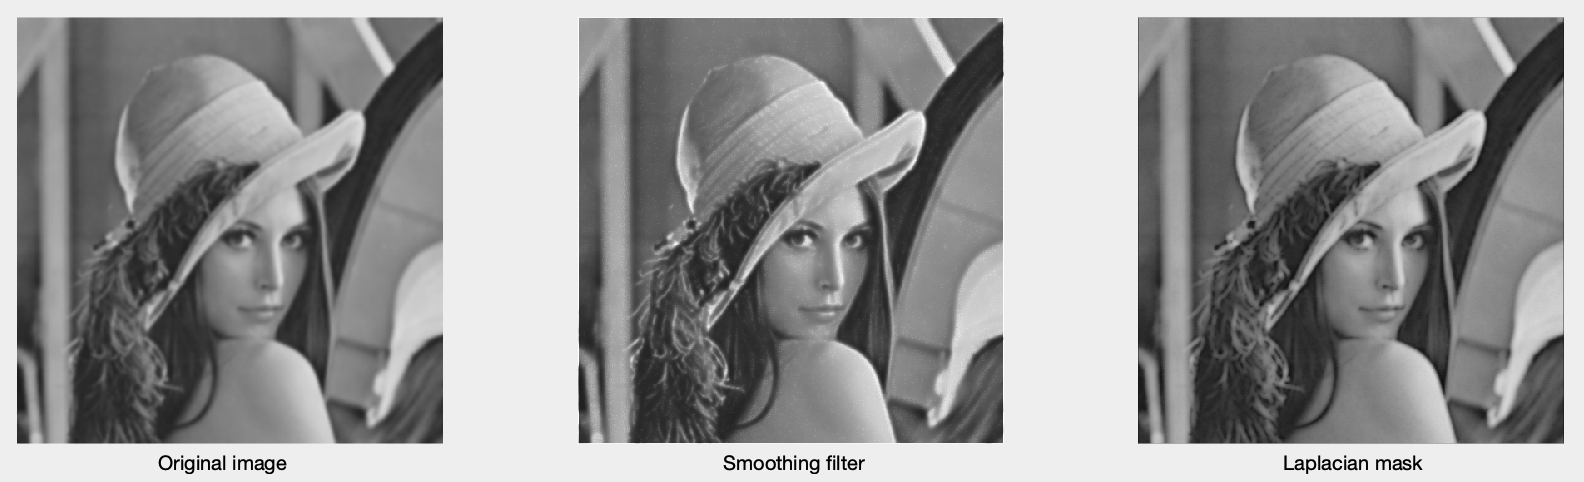
\includegraphics[width=\linewidth]{k.png}
\caption{Comparison of the original image with the sharpened images using both methods}
\label{fig:badLes}
\end{figure}

\begin{figure}[H]
\centering
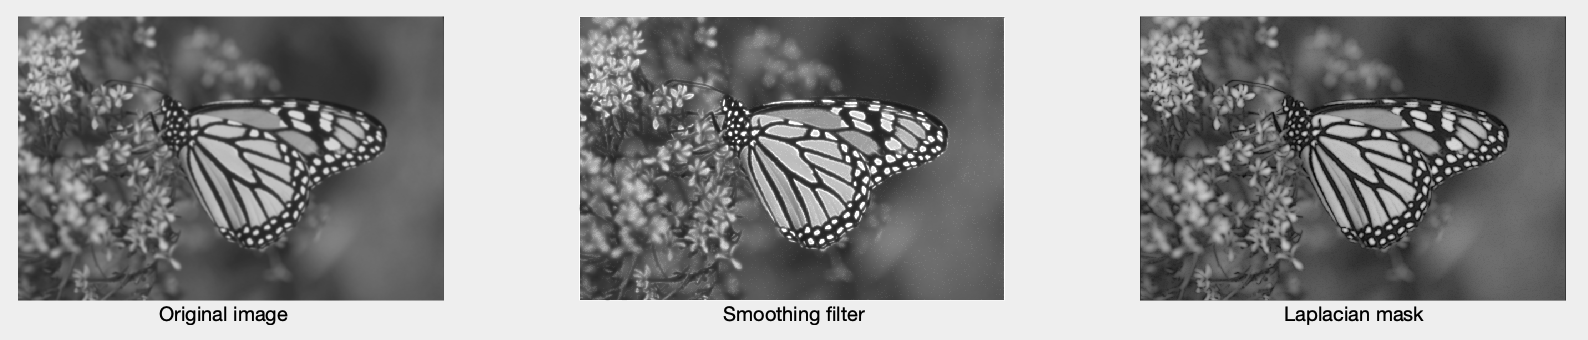
\includegraphics[width=\linewidth]{l.png}
\caption{Comparison of the original image with the sharpened images using both methods}
\label{fig:badLes}
\end{figure}

\begin{figure}[H]
\centering
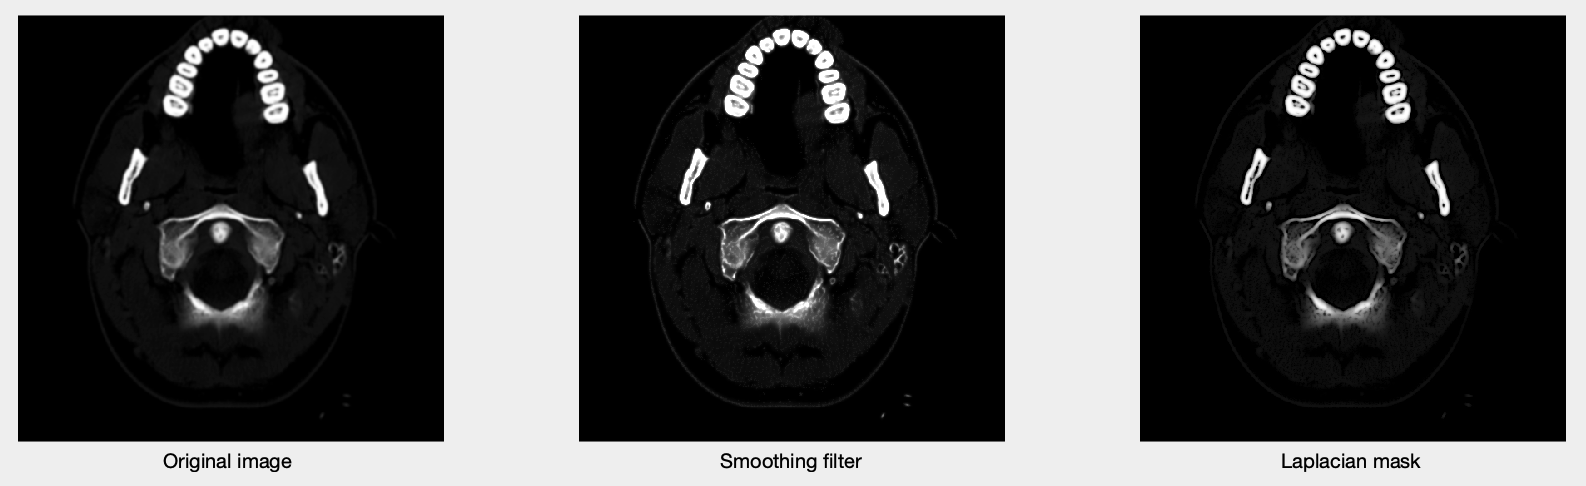
\includegraphics[width=\linewidth]{m.png}
\caption{Comparison of the original image with the sharpened images using both methods}
\label{fig:badLes}
\end{figure}

\section{Discussion}
In the first method, we had to be careful with finding the $A$ factor. It had to be high enough for us to see the difference but not too high, since sharpening artifacts appeared. In our case, that meant little white spots all over the image as seen in Figure 6.
\begin{figure}[H]
\centering
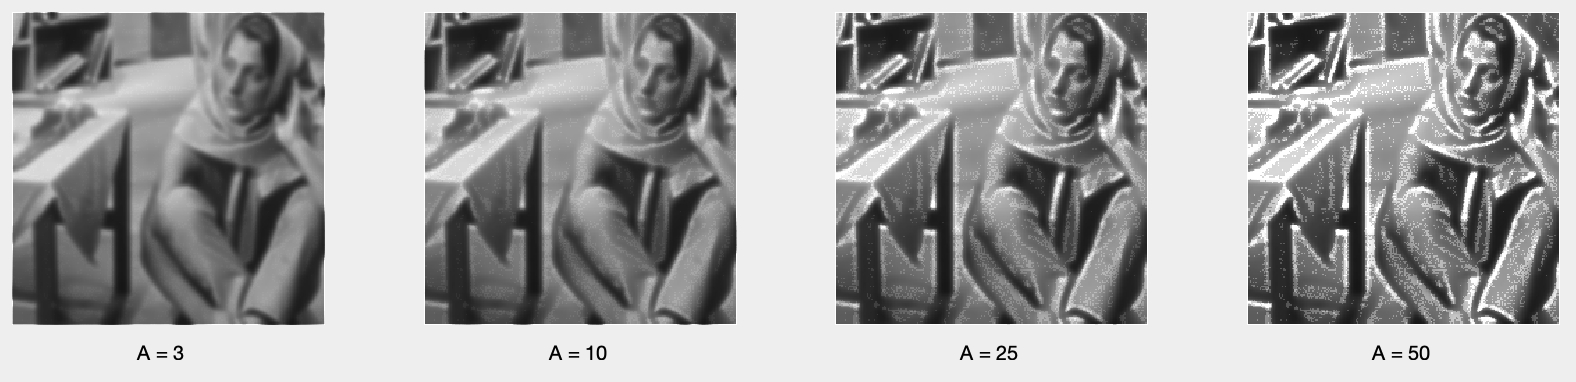
\includegraphics[width=\linewidth]{a-ji.png}
\caption{Comparison of different values of factor $A$}
\label{fig:badLes}
\end{figure}
By observing the quality of the output figure (Figure 6) we determined that $A = 10$ was the best for sharpening the image.
\newline
\newline
\\ \\
In the second method we had to choose the best Laplacian mask for sharpening. Figure 7 shows the comparison between two examples of Laplacian masks: $laPlac$ $\begin{bmatrix} 
1 & 1 & 1\\ 
1 & -8 & 1\\ 
1 & 1 & 1  
\end{bmatrix}$ and $laPlac2$ $\begin{bmatrix} 
0 & 1 & 0\\ 
1 & -4 & 1\\ 
0 & 1 & 0  
\end{bmatrix}$:

\begin{figure}[H]
\centering
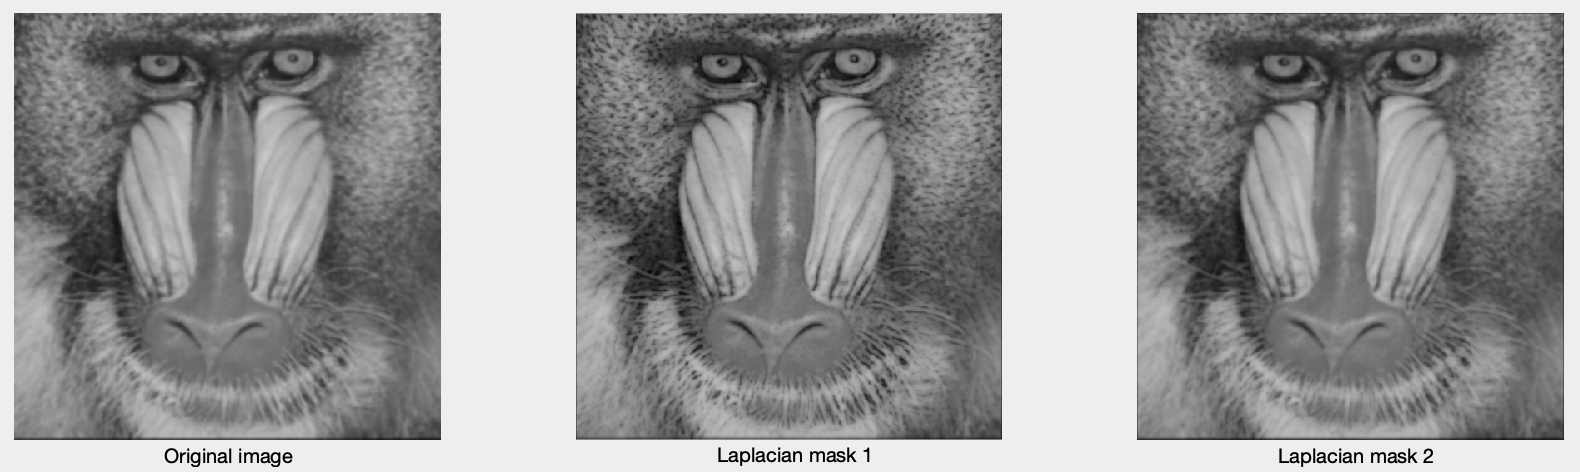
\includegraphics[width=\linewidth]{masks.png}
\caption{The difference between using the first Laplacian mask (middle image) and the second Laplacian mask (right image)}
\label{fig:badLes}
\end{figure}

By observing Figure 7 we can come to a conclusion that the first Laplacian mask is more suitable for sharpening the image, since it provides more contrast and a bigger difference than the second one.
\newline
\newline
If we compare the two utilized methods, we can note that the first method was more adjustable and it could decrease the quality of an image quicker, on the other hand, the second method had more options to choose from since we were able to apply different masks during the sharpening.

\bibliography{sample}

\begin{thebibliography}{9}

\bibitem{io} 
Wilhelm Burger, Mark J. Burge. 
\textit{Digital image processing, An Algorithmic Introduction Using Java}.
Texts in Computer Science, Springer, 2016, London.
{Accessed: 2020-12-05}

\bibitem{ena} 
MathWorks Image Processing Toolbox \texttt{https://www.mathworks.com/products/image.html}
{Accessed: 2020-12-06}

\bibitem{dva} 
$imfilter$
\texttt{https://www.mathworks.com/help/images/ref/imfilter.html}
{Accessed: 2020-12-06}

\bibitem{tri} 
$imsubtract$ \texttt{https://www.mathworks.com/help/images/ref/imsubtract.html}
{Accessed: 2020-12-06}

\bibitem{stiri} 
$imadd$ \texttt{https://www.mathworks.com/help/images/ref/imadd.html}
{Accessed: 2020-12-06}

\bibitem{con} 
$conv2$ \texttt{https://www.mathworks.com/help/matlab/ref/conv2.html}
{Accessed: 2020-12-06}

\end{thebibliography}


\end{document}
